\documentclass{beamer}
\usetheme{Dresden}
\usecolortheme{dove}
%% Checking if saving file is working more
%\usepackage{graphicx} %For jpg figure inclusion
%\usepackage{times} %For typeface
%\usepackage{epsfig}
\usepackage{color} %For Comments
\usepackage{beamerthemeshadow} %Paul and Lemmon put this in, take out if you want
%\usepackage[all]{xy}
%\usepackage{float}
%\usepackage{subfigure} 
%\usepackage{hyperref}
%\usepackage{url}
%\usepackage{parskip}
%\usepackage{multirow}

\definecolor{ForestGreen}{RGB}{34,139,34}
\definecolor{BestBlue}{RGB}{80,255,255}
% Uncomment this if you want to show work-in-progress comments
\newcommand{\comment}[1]{{\bf \tt  {#1}}}
% Uncomment this if you don't want to show comments
%\newcommand{\comment}[1]{}
\newcommand{\emcomment}[1]{\textcolor{ForestGreen}{\comment{Elena: {#1}}}}
\newcommand{\todo}[1]{\textcolor{blue}{\comment{To Do: {#1}}}}
\newcommand{\thcomment}[1]{\textcolor{BestBlue}{\comment{Thomas: {#1}}}}
\newcommand{\rmcomment}[1]{\textcolor{magenta}{\comment{Ryan: {#1}}}}
%%%%%%%%%%%%%%%%%%%%%%%%%%%%%%%%%%%%%%%%%%

\begin{document}
\author{Elena Machkasova, Thomas Hagen, Ryan McArthur}
\title{Super-fun with First-class Shapes in Quil}
\date{Clojure/conj: November 16, 2015}
\institute{University of Minnesota, Morris}


\begin{frame}
\frametitle {Super-fun with First-class Shapes in Quil}
\maketitle
\end{frame}
%frame

\begin{frame}
\frametitle{Table of contents}
\tableofcontents  
\end{frame}

\section{Overview}

\subsection{Who we are and why we are here}

\begin{frame}
\frametitle{Where are we from?}
\begin{figure}[h]
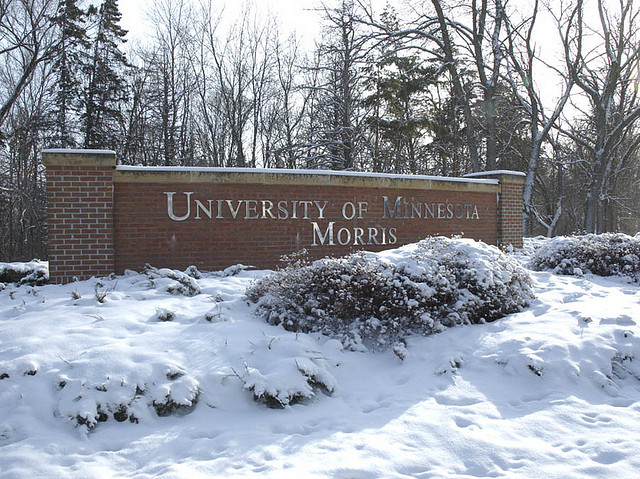
\includegraphics[width=7cm]{PresentationImages/umm-winter.jpg}
\end{figure}
UMM is a small liberal arts campus of UMN located 3 hours driving from Minneapolis/St.Paul. 
\end{frame}

\begin{frame}
\frametitle{What are we working on?}
Specific goal: developing Clojure-based introductory CS course ({\it \href{http://cda.morris.umn.edu/~elenam/\#clojure}{ClojurEd project}}). 

General goal: making Clojure more accessible to beginners and those with no Java background. 

What does this include? 
\begin{enumerate}
\item Beginner-friendly error messages. 
\item Libraries and tools that allow beginners to explore functional approaches, recursion, and abstraction.
\item Integration into a beginner-friendly IDE. 
\end{enumerate}
\end{frame}

\begin{frame}
\frametitle{What are we working on?}
Developing Clojure-based introductory CS course ({\it \href{http://cda.morris.umn.edu/~elenam/\#clojure}{ClojurEd project}}). 

General goal: making Clojure more accessible to beginners and those with no Java background. 

What does this include? 
\begin{enumerate}
\item Beginner-friendly error messages. 
\item {\bf Libraries and tools that allow beginners to explore functional approaches, recursion, and abstraction: graphical library.}
\item Integration into a beginner-friendly IDE. 
\end{enumerate}
Summer project 2015. 
\end{frame}

\subsection{Wish-list for beginner-friendly library}

\begin{frame}
\frametitle{Beginner-friendly graphical library}
Inspiration: Racket "universe" package \href{http://racket-lang.org/}{http://racket-lang.org/}
\begin{itemize}
\item Separation of Model, View, Control (MVC) 
\item Functional implementation of MVC: world state, functions: 

\noindent
old world state $\rightarrow$ new world state \\
world state $\rightarrow$ image 
\item  First-class shapes (circles, rectangles, user-added jpegs, etc) not attached to any position
\item Functions to combine simpler shapes into complex shapes: {\tt above, beside, overlay, scale...}
\end{itemize}
\end{frame}

\begin{frame}[fragile]
\frametitle{Beginner-friendly graphical library: MVC}
\begin{verbatim}
(define (main duration)
  (big-bang '() ; starts with an empty list of positions.
   [to-draw display-dots] ;draw dots on canvas
   [on-tick do-nothing 1 duration] ;dots don't move w/time
   [on-mouse add-or-remove-dot])) ;click handling
\end{verbatim}
\begin{figure}[h]
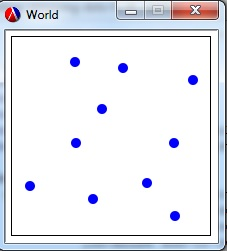
\includegraphics[width=4cm]{PresentationImages/dots.jpg}
\end{figure}
\end{frame}

\begin{frame}[fragile]
\frametitle{Beginner-friendly graphical library: first-class shapes}
\begin{verbatim}
(define dot (circle 10 "solid" "blue"))

;; display-dots: list of positions  -> image
(define (display-dots lop)     
  (cond [(empty? lop) blank-scene]
        [else (place-image dot
                           (posn-x (first lop))
                           (posn-y (first lop))
                           (display-dots (rest lop)))]))

;; add-or-remove-dot: list of positions, 
;; coordinates of click -> list of positions
.........
\end{verbatim}

\end{frame}

\begin{frame}
\frametitle{Odds and ends (not an actual slide)}
\emcomment{Don't forget:
\begin{enumerate}
\item Mention Racket influence  
\item Mention the author of Quil fun mode
\item Mention Tom Hall EuroClojure 2014
\end{enumerate}
}
\end{frame}

\begin{frame}
\frametitle{World States in Quil}
	\begin{itemize}
		\item Thanks Nikita Beloglazov for Quil Fun-Mode
		\item State as a Hash
	\end{itemize}
	\begin{figure}
		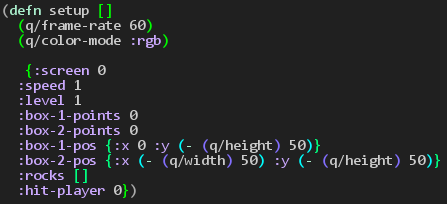
\includegraphics[width=6cm]{PresentationImages/setupCode.png}
	\end{figure}
\end{frame}

\begin{frame}
\frametitle{World States in Quil}
\begin{itemize}
		\item Elements of the state modified through functions
	\end{itemize}
	\begin{figure}
		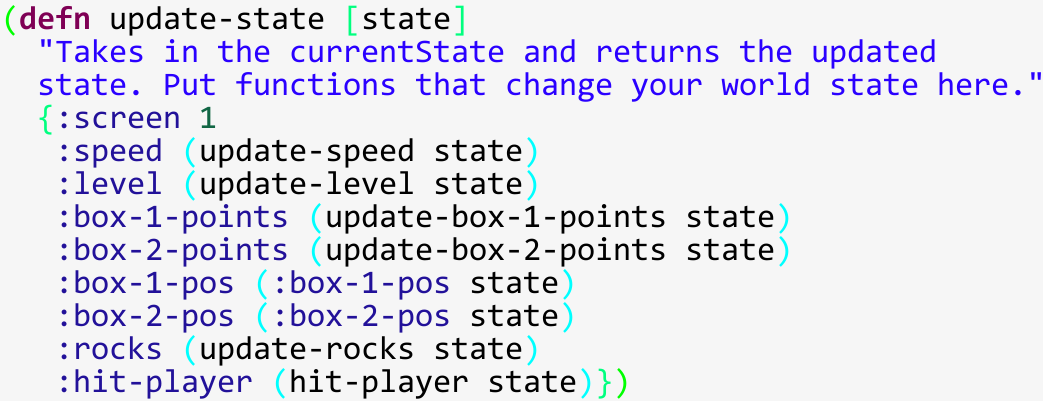
\includegraphics[width=5.5cm]{PresentationImages/updateCode.png}
		\hspace{0.1cm}
		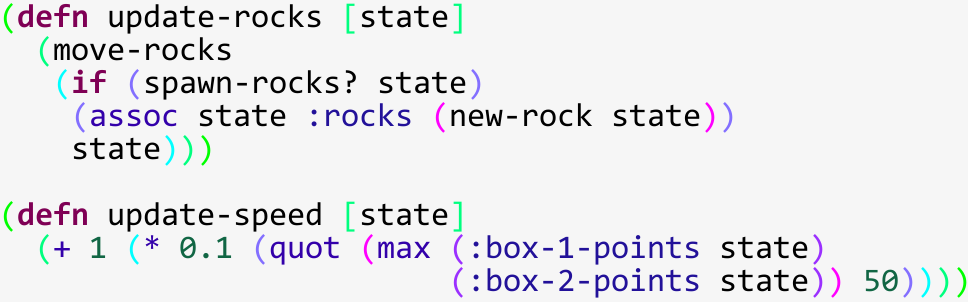
\includegraphics[width=5cm]{PresentationImages/updateFunctionsCode.png}
	\end{figure}
\end{frame}


\section{Clojure first-class shapes}

\subsection{Goals and examples}

\begin{frame}
\frametitle{Shapes as First Class Objects}
	\begin{itemize}
		\item Racket-style implementation of shapes
		\item Shapes are treated as objects, modified through functions
		\item Shapes hold their specifications for drawing
		\item Easy to redraw wherever needed
		\item Easier to understand conceptually for students
	\end{itemize}
\end{frame}

\begin{frame}
\frametitle{Creating a Collage}
	\begin{itemize}
		\item Functional Quil uses paintbrush approach
	\end{itemize}
	\begin{figure}
	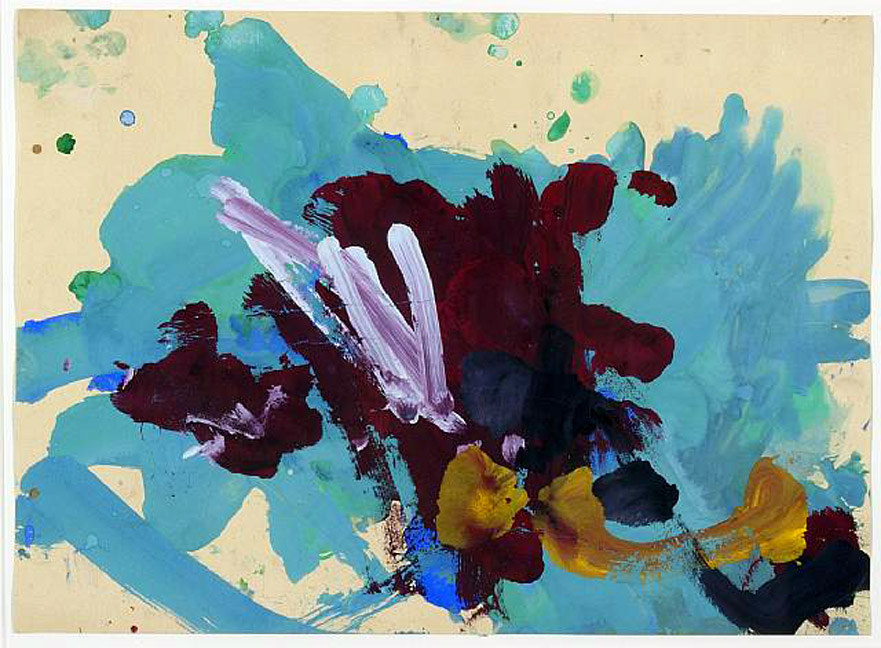
\includegraphics[width=3.5cm]{PresentationImages/painting.jpg}
	\end{figure}
	\begin{itemize}
		\item Our firstclass-shapes use collage approach
	\end{itemize}
	\begin{figure}
	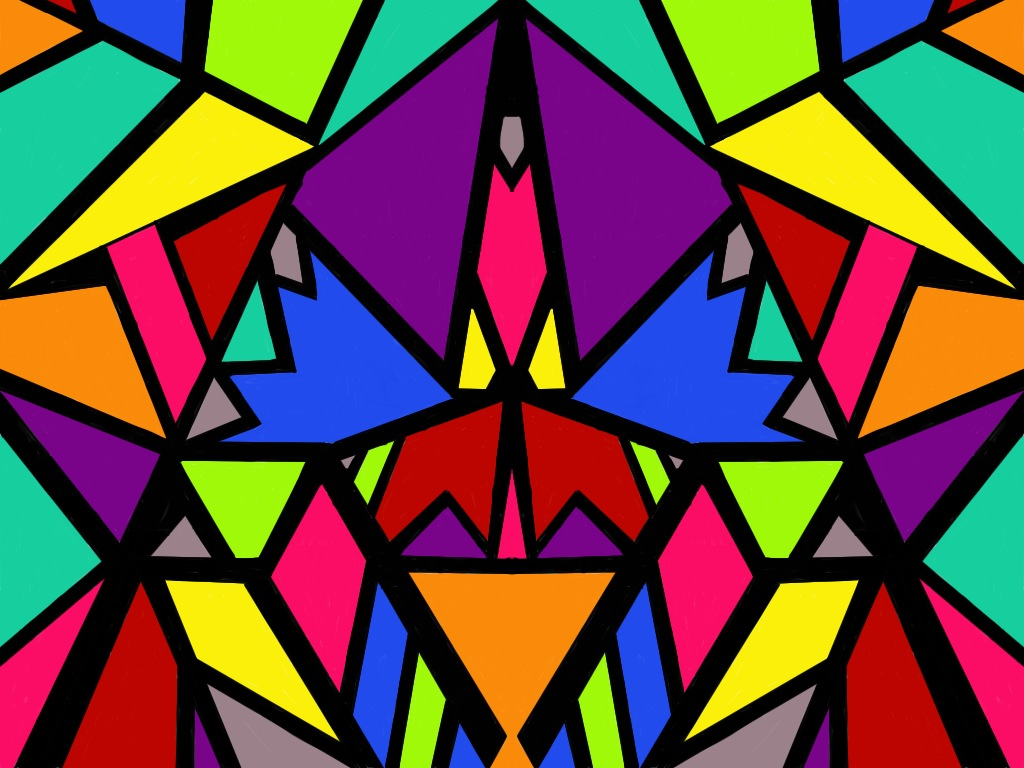
\includegraphics[width=3.5cm]{PresentationImages/collage.jpg}
	\end{figure}
\end{frame}

\begin{frame}
\frametitle{Simple Shapes}
	\begin{itemize}
		\item Quil shapes live in the draw function
		\item Quil shapes are functions to draw the shape
	\end{itemize}
	\begin{figure}
		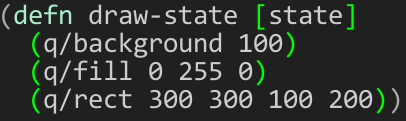
\includegraphics[width=6cm]{PresentationImages/quilGreenRect.png}
	\end{figure}
\end{frame}

\begin{frame}
\frametitle{Our Shapes}
	\begin{itemize}
		\item Our shapes are defined once in setup and reused when needed
		\item Our shapes are drawn through the draw-shape (or ds) function
	\end{itemize}
	\begin{figure}
		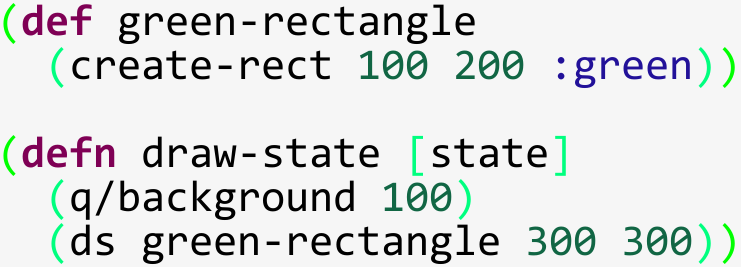
\includegraphics[width=6cm]{PresentationImages/fcsGreenRect.png}
		\hspace{1cm}
		
\includegraphics[width=1.2cm]{PresentationImages/greenRectangle.png}
	\end{figure}
\end{frame}

\begin{frame}
\frametitle{Complex Shapes}
	\begin{itemize}
		\item Complex shapes are a collection of simple shapes
		\item Each simple shape holds their individual offsets
		\item Methods are used to create complex shapes from simple ones
	\end{itemize}
	\begin{figure}
	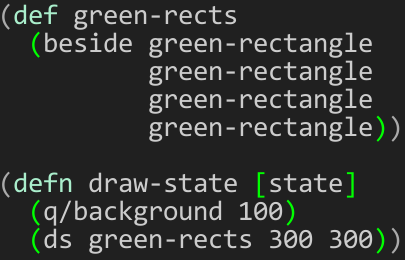
\includegraphics[width=4cm]{PresentationImages/fcsGreenRects.png}
	\hspace{1cm}
	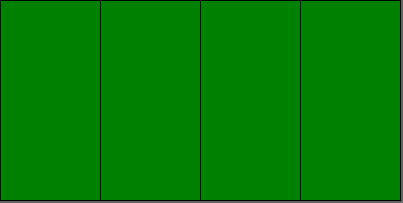
\includegraphics[width=4cm]{PresentationImages/4GreenRects.png}
	\end{figure}
\end{frame}

\begin{frame}
\frametitle{Above and Beside}
	\begin{itemize}
		\item Complex shapes are constructed through calling above or beside
		\item Can use reduce and map
	\end{itemize}
	\begin{figure}
	\vspace{-1cm}
	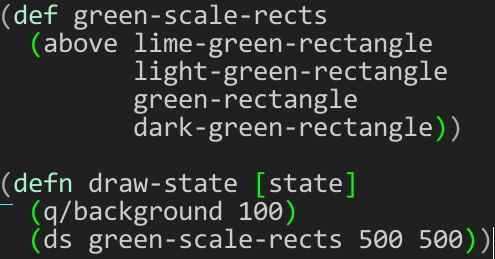
\includegraphics[width=6cm]{PresentationImages/greenScaleRects.png}
	\hspace{1.5cm}
	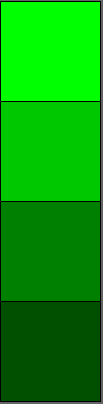
\includegraphics[width=1.2cm]{PresentationImages/greenScaleTower.png}
	\end{figure}
\end{frame}

\begin{frame}
\frametitle{Overlay}
	\begin{itemize}
		\item Complex shapes are also constructed through overlay
	\end{itemize}
	\begin{figure}
	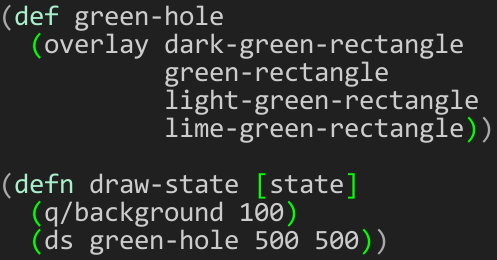
\includegraphics[width=5.5cm]{PresentationImages/fcsGreenHoleCode.png}
	\hspace{1cm}
	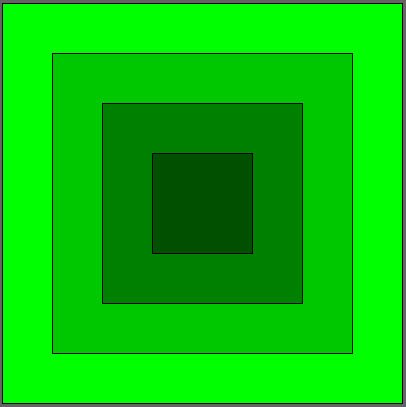
\includegraphics[width=3.5cm]{PresentationImages/greenHole.png}
	\end{figure}
\end{frame}

\begin{frame}
\frametitle{Align}
	\begin{itemize}
		\item An align version of overlay, above, and beside exist
	\end{itemize}
		\begin{figure}
		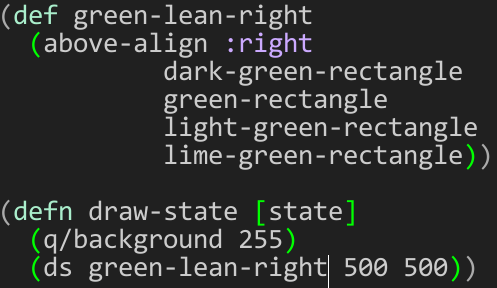
\includegraphics[width=3cm]{PresentationImages/greenLeanRightCode.png}
		\hspace{0.25cm}
		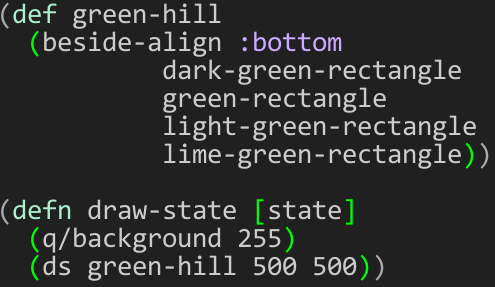
\includegraphics[width=3cm]{PresentationImages/greenSlopeBottomCode.png}
		\hspace{0.25cm}
		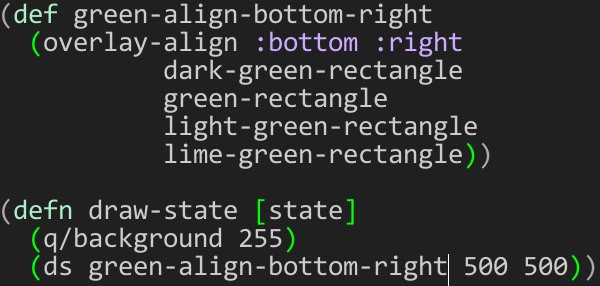
\includegraphics[width=3.65cm]{PresentationImages/greenAlignBottomRightCode.png}
	\end{figure}

	\begin{figure}
		
\includegraphics[width=1.2cm]{PresentationImages/greenLeanRight.png}
		\hspace{1cm} 	\vspace{0.3cm}
		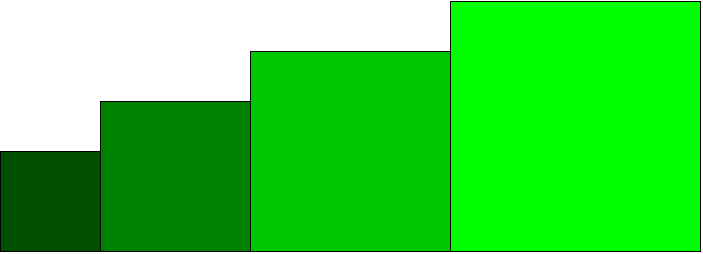
\includegraphics[width=4cm]{PresentationImages/greenSlopeBottom.png}
		\hspace{1cm} 	\vspace{0.3cm}
		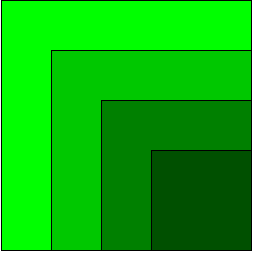
\includegraphics[width=2.5cm]{PresentationImages/greenAlignBottomRight.png}
	\end{figure}

\end{frame}

\begin{frame}[fragile]
\frametitle{Rotation and Scaling}
	\begin{itemize}
	\item You can modify the size and orientation of the shape
	\begin{columns}[t]
		\begin{column}{.45\textwidth}
			\begin{figure}[h]
				\hspace{0.25cm}
			
\includegraphics[width=4cm]{PresentationImages/rotateRedCode.png}
			\end{figure}
		\end{column}
		\begin{column}{.3\textwidth}
			\begin{figure}[h]
			
\includegraphics[width=0.8cm]{PresentationImages/red-rectangle-rotate.png}
			\end{figure}		
		\end{column}
		\end{columns}
		
		\begin{columns}[t]
		\begin{column}{.45\textwidth}
			\begin{figure}[h]
			\hspace{0.25cm}
			
\includegraphics[width=4.4cm]{PresentationImages/scaleRedCode.png}
			\end{figure}
		\end{column}
		\begin{column}{.3\textwidth}
			\begin{figure}[h]
			
\includegraphics[width=1.2cm]{PresentationImages/red-rectangle-scale.png}
			\end{figure}		
		\end{column}
		\end{columns}
		
		\begin{columns}[t]
		\begin{column}{.45\textwidth}
			\begin{figure}[h]
			\vspace{-0.5cm}
			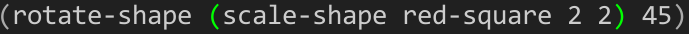
\includegraphics[width=6.5cm]{PresentationImages/rotateAndScaleRedCode.png}
			\end{figure}
		\end{column}
		\begin{column}{.3\textwidth}
			\begin{figure}[h]
			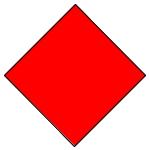
\includegraphics[width=1.7cm]{PresentationImages/red-rectangle-scale-rotate.png}
			\end{figure}		
		\end{column}
		\end{columns}
	\end{itemize}
\end{frame}

\begin{frame}
\frametitle{Code Comparison}
	\begin{itemize}
		\item Complex shapes are also constructed through overlay
	\end{itemize}
	\begin{figure}
	\hspace{-0.7cm}
	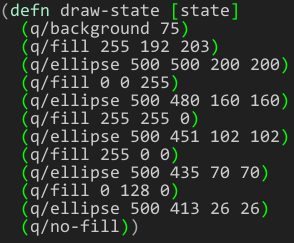
\includegraphics[width=3.5cm]{PresentationImages/theirRingsCode.png}
	\hspace{0.1cm}
	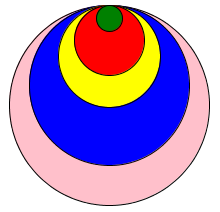
\includegraphics[width=2cm]{PresentationImages/rings.png}
	\hspace{0.1cm}
	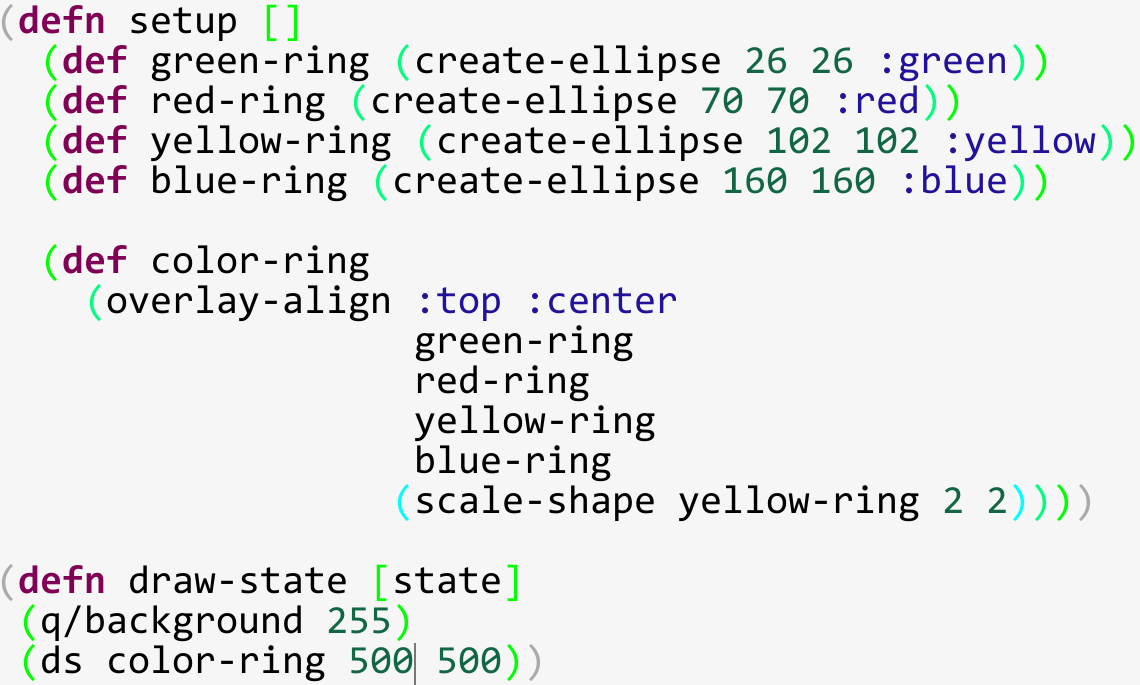
\includegraphics[width=4.5cm]{PresentationImages/ourRingsCode.png}
	\end{figure}
\end{frame}



\begin{frame}
\frametitle{Images}
	\begin{itemize}
		\item images can be rotated and scaled similar to shapes
	\end{itemize}
	\begin{figure}
		\vspace{-0.3cm}
		
\includegraphics[width=1.5cm]{PresentationImages/rich_hickey.png}
		\hspace{0.4cm}
		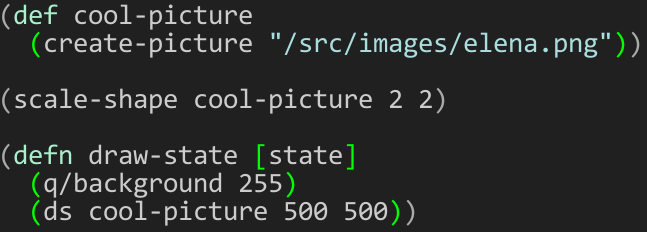
\includegraphics[width=5.5cm]{PresentationImages/pictureCode.png}
		\hspace{0.4cm}
		
\includegraphics[width=2.6cm]{PresentationImages/rich_hickey.png}
	\end{figure}

\end{frame}


\subsection{Implementation}

\begin{frame}
\frametitle{Simple Shape Structure}
	\begin{itemize}
		\item As a data structure, simple shapes are hashes
		\item Shapes hold a variety of information within them
	\end{itemize}
	\begin{figure}
		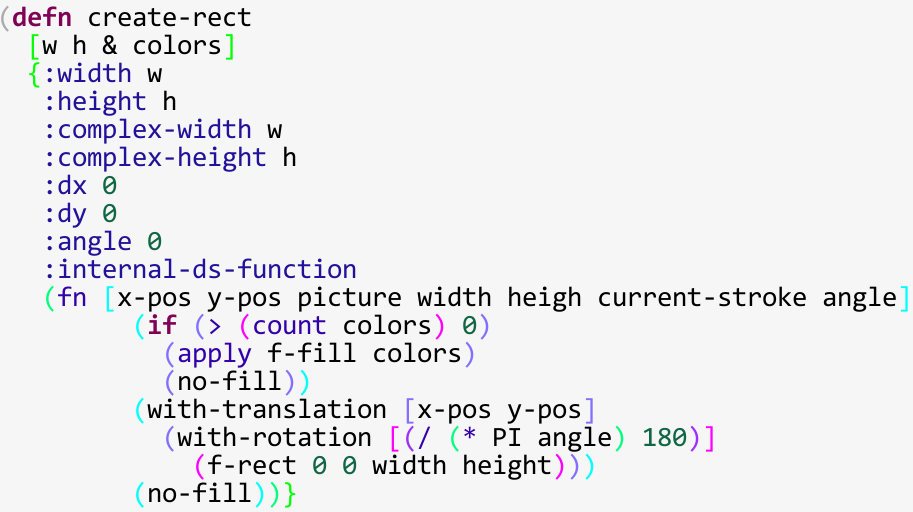
\includegraphics[width=9cm]{PresentationImages/rectHashmap.png}
	\end{figure}
\end{frame}

\begin{frame}
\frametitle{Complex Shape Structure}
	\begin{itemize}
		\item Complex shapes are vectors of shapes
		\item Each shape knows its position from the core of the shape
		\item This allows for a 'deconstructable' complex shape
	\end{itemize}
\end{frame}

\begin{frame}
\frametitle{Draw-Shape Structure}
	\begin{itemize}
		\item Draw-shape calls the internal Quil draw function within the shape object
		\item Draw-shape also works on image objects
	\end{itemize}
	\begin{figure}
		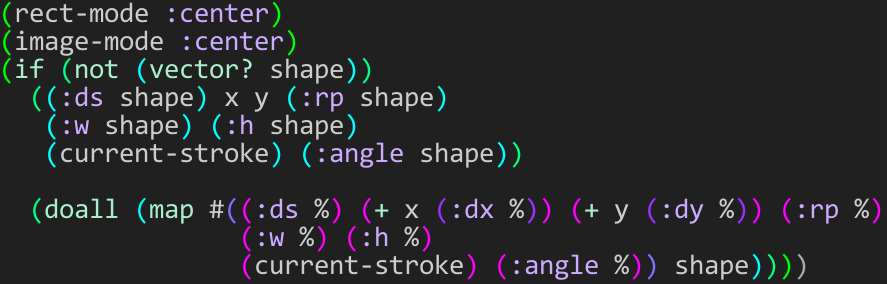
\includegraphics[width=11cm]{PresentationImages/dsCode.png}
	\end{figure}
\end{frame}

\section{Future work}

\begin{frame}
	\frametitle{Future Work}
	\begin{itemize}
		\item Fill out more functionality
		\begin{itemize}
			\item Rotate more complex shapes
			\item Pixel-detail Overlay and Overlay-Align
			\item More seamless integration with Quil fun-mode
		\end{itemize}
		\item Open Source the project
		\item Integrate a Clojure sound library
	\end{itemize}
\end{frame}

\begin{frame}
\frametitle{Acknowledgments}
	Our research was sponsored by:
	\begin{figure}
		
\includegraphics[width=10cm]{PresentationImages/logoHHMI.jpg}
	\end{figure}
	\begin{figure}
		
\includegraphics[width=10cm]{PresentationImages/logoStem.jpg}
	\end{figure}
	{\centering
	\noindent
	Thank you! \par
	Any questions? \par
	}
\end{frame}

\begin{frame}
\frametitle{Questions?}
\end{frame}
\end{document}